\section{139 - K8 - WS 1.3, WS 1.4, WS 3.4, WS 4.1 - Regentage - VerSie}

\begin{langesbeispiel} \item[6] %PUNKTE DES BEISPIELS
Medienberichten zufolge war der Sommer 2014 einer der regenreichsten Sommer seit Beginn der Wetteraufzeichnungen. Diese Behauptung wurde auch von der Tageszeitung \textit{Kurier} aufgegriffen, besonders da viele Freiluftveranstaltungen darunter zu leiden hatten. In der unten abgebildeten Grafik wurde die Anzahl der Regentage im 45-tägigen Zeitraum von 1.7.-14.8. in den Jahren 2013 und 2014 an einigen Veranstaltungsorten gegenübergestellt.

\begin{center}
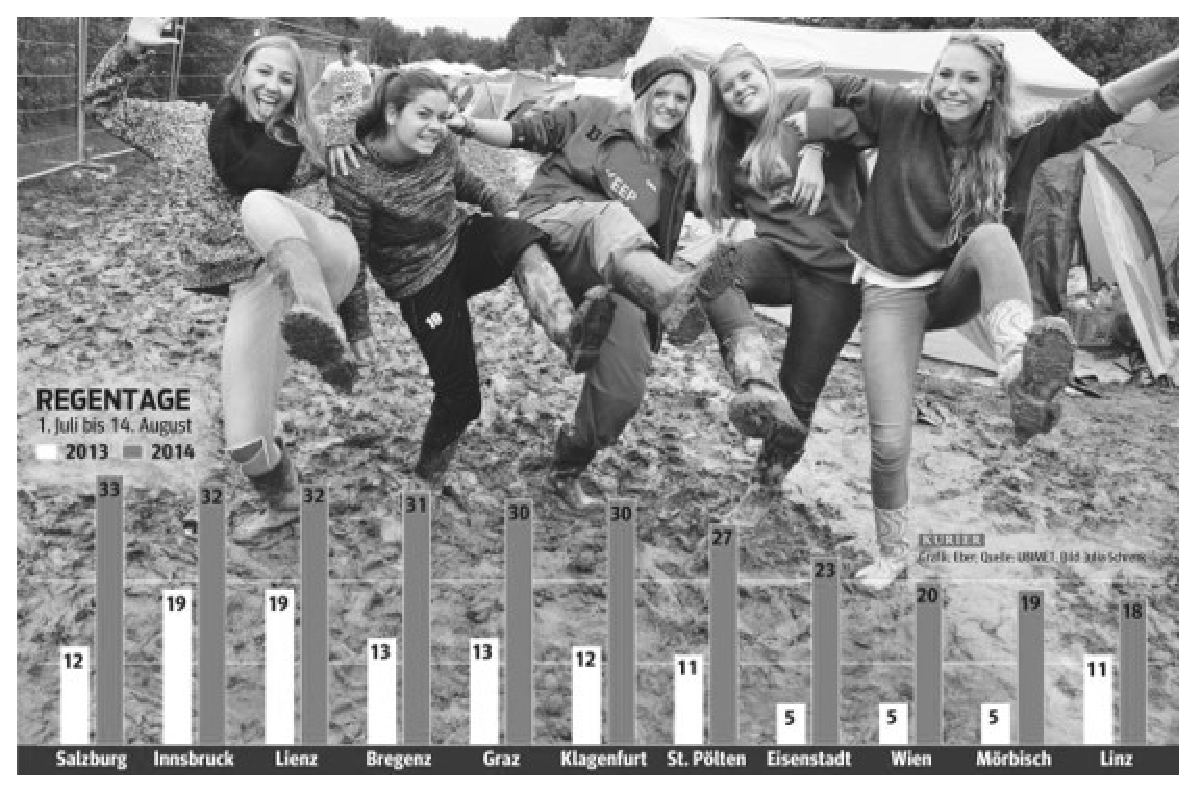
\includegraphics[width=0.8\textwidth]{../_database/Bilder/139_regentage.eps}
\end{center}%Aufgabentext

\begin{aufgabenstellung}
\item %Aufgabentext

\ASubitem{Gib das arithmetische Mittel und den Median für die Anzahl der Regentage im Sommer 2014 an.} %Unterpunkt1
\Subitem{Gib an, welcher dieser beiden Werte sich stärker ändert, wenn man Mörbisch und Lienz weglässt und das arithmetische Mittel und den Median für die Anzahl der Regentage nur in den Landeshauptstädten berechnet. Begründe deine Entscheidung.} %Unterpunkt2

\item %Aufgabentext

\Subitem{Aus den gegebenen Werten ergibt sich für die Anzahl der Regentage im Jahr 2014 die relative Häufigkeit $0,594$. Bestimme daraus für den genannten Zeitraum näherungsweise ein 95\,\% Konfidenzintervall für die Anzahl der Regentage 2014 an einem beliebigen Ort.} %Unterpunkt1
\Subitem{Ändere einen Parameter so, dass bei gleicher relativer Häufigkeit die Schätzung genauer wird.} %Unterpunkt2

\item Ein Reiseführer für Österreich gibt an, dass die Wahrscheinlichkeit für einen Regentag in Österreich bei ca. 41\,\% liegt. Lena möchte ein Semester mit 122 Tagen in Österreich studieren und diverse Veranstaltungen besuchen. Die Zufallsvariable $X$ beschreibt die Anzahl der Regentage und kann durch die Normalverteilung approximiert werden. Der abgebildete Graph bildet die zugehörige Dichtefunktion ab.
	
	\begin{center}
	\psset{xunit=0.25cm,yunit=50cm,algebraic=true,dimen=middle,dotstyle=o,dotsize=5pt 0,linewidth=1.6pt,arrowsize=3pt 2,arrowinset=0.25}
\begin{pspicture*}(22.857618000000016,-0.01)(77.18238200000003,0.07691370902045518)
\psaxes[labelFontSize=\scriptstyle,xAxis=true,yAxis=true,Dx=2.,Dy=0.01,ticksize=-2pt 0,subticks=0]{->}(0,0)(22.857618000000016,-0.0037698070915797434)(77.18238200000003,0.07691370902045518)[$X$,140] [,-40]
\pscustom[linewidth=0.8pt,fillcolor=black,fillstyle=solid,opacity=0.5]{\psplot{55.00098623685058}{78.182382}{EXP((-(x-50.02)^(2.0))/(5.4324764^(2.0)*2.0))/(abs(5.4324764)*sqrt(3.141592653589793*2.0))}\lineto(78.182382,0)\lineto(55.00098623685058,0)\closepath}
\psplot[linewidth=1.6pt,plotpoints=200]{22.857618000000016}{77.18238200000003}{EXP((-(x-50.02)^(2.0))/(5.4324764^(2.0)*2.0))/(abs(5.4324764)*sqrt(3.141592653589793*2.0))}
\rput[tl](55,0.0592134861073945){$\varphi(X)$}
\begin{scriptsize}
\psdots[dotsize=4pt 0,dotstyle=triangle*](78.182382,0.)
\end{scriptsize}
\end{pspicture*}
	\end{center}%Aufgabentext

\Subitem{Berechne, welchen Anteil die markierte Fläche von der Gesamtfläche einnimmt.} %Unterpunkt1
\Subitem{Interpretiere das Ergebnis im gegebenen Zusammenhang.} %Unterpunkt2

\end{aufgabenstellung}

\begin{loesung}
\item \subsection{Lösungserwartung:} 

\Subitem{Arithmetisches Mittel: $\dfrac{33+32+32+31+30+30+27+23+20+19+18}{11}=\dfrac{295}{11}=26,\overline{81}$
	
	Median: 30} %Lösung von Unterpunkt1
\Subitem{Ohne Mörbisch und Lienz:
	
	Arithmetische Mittel: $\dfrac{33+32+31+30+30+27+23+20+18}{11}=\dfrac{244}{9}=27,\dot{1}$
	
	Median: 30
	
	Da ein Wert "`über"' und ein Wert "`unter"' dem Median weggenommen worden ist, bleibt der Median unverändert. Das arithmetische Mittel wird größer, da Mörbisch 7,81 Regentage weniger als das arithmetische Mittel hatte, Lienz aber "`nur"' 5,19 Regentage mehr.} %%Lösung von Unterpunkt2

\setcounter{subitemcounter}{0}
\subsection{Lösungsschlüssel:}
 
\Subitem{Ein Punkt für die richtige Berechnung des arithemtischen Mittels und des Medians.} %Lösungschlüssel von Unterpunkt1
\Subitem{Ein Punkt für den richtige Begründung.} %Lösungschlüssel von Unterpunkt2

\item \subsection{Lösungserwartung:} 

\Subitem{Toleranzintervall: $[0,4505177847; 0,7374822153]$
	
	Anzahl der Regentage: $[20,2733; 33,1866] \Rightarrow [20;34]$} %Lösung von Unterpunkt1
\Subitem{Da der Zeitraum fest vorgegeben ist, man also die Anzahl der Tage nicht verändern kann, muss das Sicherheitsniveau kleiner werden um eine genauere Schätzung zu erhalten.} %%Lösung von Unterpunkt2

\setcounter{subitemcounter}{0}
\subsection{Lösungsschlüssel:}
 
\Subitem{Ein Punkt für die richtigen Regentage.} %Lösungschlüssel von Unterpunkt1
\Subitem{Ein Punkt für die richtige Änderung eines Parameters.} %Lösungschlüssel von Unterpunkt2

\item \subsection{Lösungserwartung:} 

\Subitem{$\mu=50,02; \sigma=5,43248 \Rightarrow P(X\geq 55)=0,1796=17,96\,\%$} %Lösung von Unterpunkt1
\Subitem{Die Fläche gibt die Wahrscheinlichkeit an, dass Lena in ihrem Auslandssemester mindestens 55 Regentage erlebt.} %%Lösung von Unterpunkt2

\setcounter{subitemcounter}{0}
\subsection{Lösungsschlüssel:}
 
\Subitem{Ein Punkt für die korrekte Berechnung der Wahrscheinlichkeit.} %Lösungschlüssel von Unterpunkt1
\Subitem{Ein Punkt für die korrekte Interpretation.} %Lösungschlüssel von Unterpunkt2

\end{loesung}

\end{langesbeispiel}